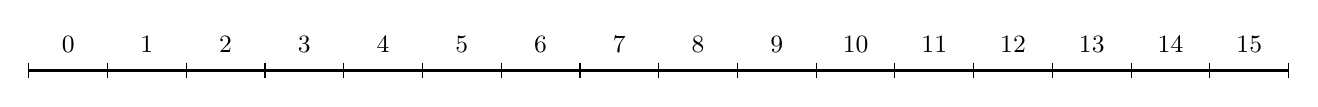
\begin{tikzpicture}
% Total segment length and number of divisions
\def\length{16}  % cm
\def\divisions{16}
\def\step{\length/\divisions}

% Draw main segment
\draw[thick] (0,0) -- (\length,0);

% Draw division ticks
\foreach \i in {0,...,\divisions} {
    \draw[thin] ({\i*\step},0.1) -- ({\i*\step},-0.1); % Vertical tick mark
}

% Draw interval labels centered between ticks
\foreach \i in {0,...,15} {
    \node[anchor=south] at ({(\i+0.5)*\step},0.1) {\small \i};
}

\end{tikzpicture}
